\documentclass[12pt]{beamer}
\usepackage{../Estilos/BeamerMAF}
%Sección para el tema de beamer, con el theme, usercolortheme y sección de footers
\usetheme{CambridgeUS}
\usecolortheme{beaver}
%\useoutertheme{default}
\setbeamercovered{invisible}
% or whatever (possibly just delete it)
\setbeamertemplate{section in toc}[sections numbered]
\setbeamertemplate{subsection in toc}[subsections numbered]
\setbeamertemplate{subsection in toc}{\leavevmode\leftskip=3.2em\rlap{\hskip-2em\inserttocsectionnumber.\inserttocsubsectionnumber}\inserttocsubsection\par}
\setbeamercolor{section in toc}{fg=blue}
\setbeamercolor{subsection in toc}{fg=blue}
\setbeamercolor{frametitle}{fg=blue}
\setbeamertemplate{caption}[numbered]

\setbeamertemplate{footline}
\beamertemplatenavigationsymbolsempty
\setbeamertemplate{headline}{}


\makeatletter
\setbeamercolor{section in foot}{bg=gray!30, fg=black!90!orange}
\setbeamercolor{subsection in foot}{bg=blue!30!yellow, fg=red}
\setbeamercolor{date in foot}{bg=black, fg=white}
\setbeamertemplate{footline}
{
  \leavevmode%
  \hbox{%
  \begin{beamercolorbox}[wd=.333333\paperwidth,ht=2.25ex,dp=1ex,center]{section in foot}%
    \usebeamerfont{section in foot} \insertsection
  \end{beamercolorbox}%
  \begin{beamercolorbox}[wd=.333333\paperwidth,ht=2.25ex,dp=1ex,center]{subsection in foot}%
    \usebeamerfont{subsection in foot}  \insertsubsection
  \end{beamercolorbox}%
  \begin{beamercolorbox}[wd=.333333\paperwidth,ht=2.25ex,dp=1ex,right]{date in head/foot}%
    \usebeamerfont{date in head/foot} \insertshortdate{} \hspace*{2em}
    \insertframenumber{} / \inserttotalframenumber \hspace*{2ex} 
  \end{beamercolorbox}}%
  \vskip0pt%
}
\makeatother\newlength{\depthofsumsign}
\setlength{\depthofsumsign}{\depthof{$\sum$}}
\newcommand{\nsum}[1][1.4]{% only for \displaystyle
    \mathop{%
        \raisebox
            {-#1\depthofsumsign+1\depthofsumsign}
            {\scalebox
                {#1}
                {$\displaystyle\sum$}%
            }
    }
}
\def\scaleint#1{\vcenter{\hbox{\scaleto[3ex]{\displaystyle\int}{#1}}}}
\def\bs{\mkern-12mu}





%\RequirePackage{currfile}
\documentclass[12pt]{beamer}
\usepackage[utf8]{inputenc}
\usepackage[spanish]{babel}
\usepackage{standalone}
\usepackage{color}
\usepackage{siunitx}
\usepackage{hyperref}
\usepackage[outdir=./]{epstopdf}
%\hypersetup{colorlinks,linkcolor=,urlcolor=blue}
%\hypersetup{colorlinks,urlcolor=blue}
\usepackage{xcolor,soul}
\usepackage{etoolbox}
\usepackage{amsmath}
\usepackage{amsthm}
\usepackage{mathtools}
\usepackage{tcolorbox}
\usepackage{physics}
\usepackage{multicol}
\usepackage{bookmark}
\usepackage{longtable}
\usepackage{listings}
\usepackage{cancel}
\usepackage{wrapfig}
\usepackage{empheq}
\usepackage{graphicx}
\usepackage{tikz}
\usetikzlibrary{calc, patterns, matrix, backgrounds, decorations,shapes, arrows.meta}
\usepackage[autostyle,spanish=mexican]{csquotes}
\usepackage[os=win]{menukeys}
\usepackage{pifont}
\usepackage{pbox}
\usepackage{bm}
\usepackage{caption}
\captionsetup{font=scriptsize,labelfont=scriptsize}
%\usepackage[sfdefault]{roboto}  %% Option 'sfdefault' only if the base font of the document is to be sans serif

%Sección de definición de colores
\definecolor{ao}{rgb}{0.0, 0.5, 0.0}
\definecolor{bisque}{rgb}{1.0, 0.89, 0.77}
\definecolor{amber}{rgb}{1.0, 0.75, 0.0}
\definecolor{armygreen}{rgb}{0.29, 0.33, 0.13}
\definecolor{alizarin}{rgb}{0.82, 0.1, 0.26}
\definecolor{cadetblue}{rgb}{0.37, 0.62, 0.63}
\definecolor{deepblue}{rgb}{0,0,0.5}
\definecolor{brown}{rgb}{0.59, 0.29, 0.0}
\definecolor{OliveGreen}{rgb}{0,0.25,0}
\definecolor{mycolor}{rgb}{0.122, 0.435, 0.698}

\newcommand*{\boxcolor}{orange}
\makeatletter
\newcommand{\boxedcolor}[1]{\textcolor{\boxcolor}{%
\tikz[baseline={([yshift=-1ex]current bounding box.center)}] \node [rectangle, minimum width=1ex, thick, rounded corners,draw] {\normalcolor\m@th$\displaystyle#1$};}}
 \makeatother

\newtcbox{\mybox}{on line,
  colframe=mycolor,colback=mycolor!10!white,
  boxrule=0.5pt,arc=4pt,boxsep=0pt,left=6pt,right=6pt,top=6pt,bottom=6pt}

\usefonttheme[onlymath]{serif}
%Sección de definición de nuevos comandos

\newcommand*{\TitleParbox}[1]{\parbox[c]{1.75cm}{\raggedright #1}}%
\newcommand{\python}{\texttt{python}}
\newcommand{\textoazul}[1]{\textcolor{blue}{#1}}
\newcommand{\azulfuerte}[1]{\textcolor{blue}{\textbf{#1}}}
\newcommand{\funcionazul}[1]{\textcolor{blue}{\textbf{\texttt{#1}}}}
\newcommand{\ptilde}[1]{\ensuremath{{#1}^{\prime}}}
\newcommand{\stilde}[1]{\ensuremath{{#1}^{\prime \prime}}}
\newcommand{\ttilde}[1]{\ensuremath{{#1}^{\prime \prime \prime}}}
\newcommand{\ntilde}[2]{\ensuremath{{#1}^{(#2)}}}
\renewcommand{\arraystretch}{1.5}

\newcounter{saveenumi}
\newcommand{\seti}{\setcounter{saveenumi}{\value{enumi}}}
\newcommand{\conti}{\setcounter{enumi}{\value{saveenumi}}}
\renewcommand{\rmdefault}{cmr}% cmr = Computer Modern Roman

\linespread{1.5}

\usefonttheme{professionalfonts}
%\usefonttheme{serif}
\DeclareGraphicsExtensions{.pdf,.png,.jpg}


%Sección para el tema de beamer, con el theme, usercolortheme y sección de footers
\mode<presentation>
{
  \usetheme{CambridgeUS}
  
  %\useoutertheme{infolines}
  \useoutertheme{default}
  \usecolortheme{beaver}
  \setbeamercovered{invisible}
  % or whatever (possibly just delete it)
  \setbeamertemplate{section in toc}[sections numbered]
  \setbeamertemplate{subsection in toc}[subsections numbered]
  \setbeamertemplate{subsection in toc}{\leavevmode\leftskip=3.2em\rlap{\hskip-2em\inserttocsectionnumber.\inserttocsubsectionnumber}\inserttocsubsection\par}
  \setbeamercolor{section in toc}{fg=blue}
  \setbeamercolor{subsection in toc}{fg=blue}
  \setbeamercolor{frametitle}{fg=blue}
  \setbeamertemplate{caption}[numbered]

  \setbeamertemplate{footline}
  \beamertemplatenavigationsymbolsempty
  \setbeamertemplate{headline}{}
}

\makeatletter
\setbeamercolor{section in foot}{bg=gray!30, fg=black!90!orange}
\setbeamercolor{subsection in foot}{bg=blue!30!yellow, fg=red}
\setbeamertemplate{footline}
{
  \leavevmode%
  \hbox{%
  \begin{beamercolorbox}[wd=.333333\paperwidth,ht=2.25ex,dp=1ex,center]{section in foot}%
    \usebeamerfont{section in foot} \insertsection
  \end{beamercolorbox}}%
  \begin{beamercolorbox}[wd=.333333\paperwidth,ht=2.25ex,dp=1ex,center]{subsection in foot}%
    \usebeamerfont{subsection in foot}  \insertsubsection
  \end{beamercolorbox}%
  \begin{beamercolorbox}[wd=.333333\paperwidth,ht=2.25ex,dp=1ex,right]{date in head/foot}%
    \usebeamerfont{date in head/foot} \insertshortdate{} \hspace*{2em}
    \insertframenumber{} / \inserttotalframenumber \hspace*{2ex} 
  \end{beamercolorbox}}%
  \vskip0pt%
\makeatother  

\makeatletter
\patchcmd{\beamer@sectionintoc}
  {\vfill}
  {\vskip\itemsep}
  {}
  {}
\makeatother


\newcommand{\Cancel}[2][black]{{\color{#1}\cancel{\color{black}#2}}}
\title{\large{Asesoría Separación de variables}}
\author{M. en C. Gustavo Contreras Mayén}
\date{}
% \institute{Facultad de Ciencias - UNAM}
% \titlegraphic{
\includegraphics[width=1.75cm]{../Imagenes/escudo-facultad-ciencias}\hspace*{4.75cm}~%
%    
\includegraphics[width=1.75cm]{../Imagenes/escudo-unam}
% }
\setbeamertemplate{navigation symbols}{}
\begin{document}
\maketitle
\fontsize{14}{14}\selectfont
\spanishdecimal{.}
\section*{Contenido}
\frame{\tableofcontents[currentsection, hideallsubsections]}

%Ref. Zamora (2012) - Notas EDP 2.1.6 Lámina rectangular
\section{Ecuación de calor en un lámina rectangular}
\frame{\tableofcontents[currentsection, hideothersubsections]}
\subsection{Planteamiento del problema}

\begin{frame}
\frametitle{El problema a resolver}
Consideremos el problema de \emph{conducción de calor en dos dimensiones} en un sistema cartesiano:
\begin{align}
u_{t} = \alpha^{2} \, \laplacian{u}
\label{eq:ecuacion_02_187}
\end{align}
\end{frame}

\subsection{Condiciones de frontera e iniciales}

\begin{frame}
\frametitle{Condiciones de Frontera}
Con las condiciones de frontera (CDF):
\begin{align}
u(0, y, t) &= 0 \label{eq:ecuacion_02_188} \\
u(a, y, t) &= 0 \label{eq:ecuacion_02_189} \\
u(x, 0, t) &= 0 \label{eq:ecuacion_02_190} \\
u(x, b, t) &= 0 \label{eq:ecuacion_02_191} \\
0 < t &< \infty \nonumber
\end{align}
\end{frame}
\begin{frame}
\frametitle{Condiciones iniciales}
Y las condiciones iniciales (CI):
\begin{align}
u(x, y, 0) = f (x, y) \label{eq:ecuacion_02_192}
\end{align}
definido para $0 < x < a$, $0  < y < b$ y $t > 0$.
\end{frame}
\begin{frame}
\frametitle{Esquema del problema}
\begin{figure}[H]
    \centering
    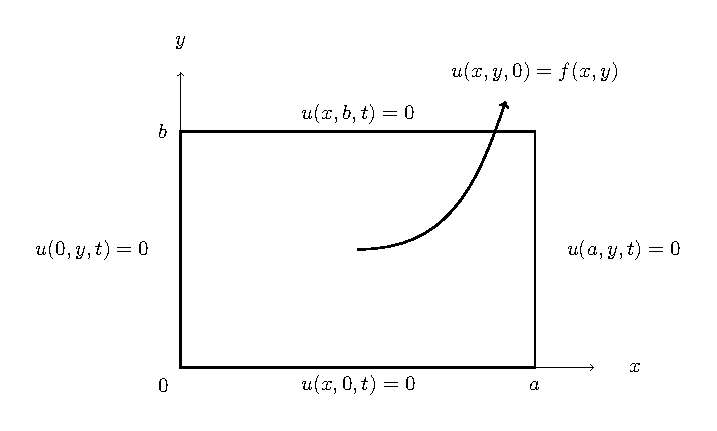
\includegraphics[scale=0.9]{Imagenes/Separacion_Variables_01_Lamina_Cuad.eps}
    \caption{Región de una lámina cuadrada para resolver el problema.}
    \label{fig:figura_lamina_cuadrada}
\end{figure}
\end{frame}
\begin{frame}
\frametitle{Ocupando el operador laplaciano}
Ocuparemos la definición del operador de Laplace o Laplaciano en dos dimensiones $x$, $y$:
\begin{align}
\laplacian{u} = u_{xx} + u_{yy}
\label{eq:ecuacion_02_193}
\end{align}
Nótese que, a pesar que $u$ es función tanto de $(x, y) $ como de $t$, el Laplaciano sólo actúa en las coordenadas espaciales.
\end{frame}
\begin{frame}
\frametitle{Entendiendo el problema}
Podemos interpretar este problema como la difusión de calor a través de la frontera de la lámina rectangular $[ 0, a ] \cp [ 0, b ]$ cuando esta lámina se encuentra aislada térmicamente tanto en su área superior como en su área inferior, como se aprecia en la fig (\ref{fig:figura_lamina_cuadrada}).
\end{frame}
\begin{frame}
\frametitle{Las condiciones de frontera}
Las condiciones de frontera (\ref{eq:ecuacion_02_188})-(\ref{eq:ecuacion_02_191}) para este problema especifican una temperatura constante cero en todo el perímetro del rectángulo.
\end{frame}

\subsection{Separación de variables}

\begin{frame}
\frametitle{Separación de variables}
La propuesta de solución para la técnica de separación de variables es para este caso:
\begin{align}
u (x, y, t) = X(x) \, Y(y) \, T(t)
\label{eq:ecuacion_02_194}
\end{align}
\pause
Recordemos que cada función con mayúscula depende de una sola variable.
\end{frame}
\begin{frame}
\frametitle{Calculando derivadas parciales}
Calculamos las derivadas parciales que habrá que sustituir en la ecuación (\ref{eq:ecuacion_02_194}):
\begin{align*}
u_{t} &= X(x) \, Y(y) \, \ptilde{T} (t) \\[0.5em]
u_{xx} &= \stilde{X} (x) \, Y(y) \, T(t) \\[0.5em]
u_{yy} &= X(x) \, \stilde{Y} (y) \, T(t)
\end{align*}
\end{frame}
\begin{frame}
\frametitle{Acomodando los términos}
Por lo que tendremos:
\begin{align*}
X(x) \, Y(y) \, \ptilde{T} (t) &= \alpha^{2} \bigg[ \stilde{X} (x) \, Y(y) \, T(t) + \\[0.5em]
&+ X(x) \, \stilde{Y} (y) \, T(t) \bigg]
\end{align*}
\pause
Continuamos con el siguiente paso que es dividir entre la solución propuesta.
\end{frame}
\begin{frame}
\frametitle{Avanzando en la separación de variables}
Ahora dividimos entre $X(x) \, Y(y) \, T(t)$, obteniendo:
\pause
\begin{align*}
\dfrac{\ptilde{T}(t)}{T(t)} = \alpha^{2} \left[ \dfrac{\stilde{X}(x)}{X(x)} + \dfrac{\ptilde{Y}(y)}{Y(y)} \right]
\end{align*}
\pause
En donde encontramos que la expresión del lado izquierdo de la igualdad depende solo de la variable $t$, mientras que la expresión del lado derecho depende tanto de $x$ e $y$.
\end{frame}
\begin{frame}
\frametitle{Primera constante de separación}
Como $t$, $x$, $y$ son variables independientes, la igualdad solo puede ser posible si ambas funciones son iguales a una función constante.
\pause
\begin{align*}
\dfrac{\ptilde{T}(t) }{T(t)} =  \alpha^{2} \left[ \dfrac{\stilde{X}(x)}{X(x)} + \dfrac{\ptilde{Y}(y)}{Y(y)} \right] = A
\end{align*}
\pause
Donde $A$ es una constante por determinar.
\end{frame}
\begin{frame}
\frametitle{Primera EDO}
Tendremos entonces la primera EDO:
\begin{align}
\ptilde{T}(t) - A \, T(t) = 0
\label{eq:ecuacion_02_195}
\end{align}
\pause
Del curso de EDO I, ya tenemos una idea de cómo resolver esta ecuación, quedando pendiente definir primera constante de separación $A$.
\end{frame}
\begin{frame}
\frametitle{Segunda constante de separación}
Tomando por separado la igualdad del lado derecho, tendremos una segunda constante de separación:
\pause
\begin{align*}
\left[ \dfrac{\stilde{X}(x)}{X(x)} + \dfrac{\ptilde{Y}(y)}{Y(y)} \right]  = \dfrac{A}{\alpha^{2}} = B
\end{align*}
\end{frame}
\begin{frame}
\frametitle{Continuando con la separación de variables}
Avanzando en la revisión del término para las variables $x$ e $y$, se tiene que:
\pause
\begin{align*}
\dfrac{\stilde{X}(x)}{X(x)} = -  \dfrac{\ptilde{Y}(y)}{Y(y)} = C
\end{align*}
\pause
y además
\begin{align*}
\dfrac{\ptilde{Y}(y)}{Y(y)} = D
\end{align*}
Tal que: $B = C+ D$
\end{frame}
\begin{frame}
\frametitle{Las otras EDO}
Entonces tendremos las siguientes EDO:
\begin{align}
\stilde{X}(x) - C \, X(x) = 0 \label{eq:ecuacion_02_196} \\[0.5em]
\stilde{Y}(y) - D \, Y(y) = 0 \label{eq:ecuacion_02_197}
\end{align}
con $A$, $B$, $C$ y $D$ constantes que satisfacen $B = C + D$ y $B = A / \alpha^{2}$
\end{frame}
\begin{frame}
\frametitle{Las CDF}
Recordemos que las condiciones de frontera son:
\begin{align}
X(0) &= 0 \label{eq:ecuacion_02_198} \\[0.5em]
X(a) &= 0 \label{eq:ecuacion_02_199} \\[0.5em]
Y(0) &= 0 \label{eq:ecuacion_02_200} \\[0.5em]
Y(b) &= 0 \label{eq:ecuacion_02_201}
\end{align}
\end{frame}

\subsection{Solución a las EDO}

\begin{frame}
\frametitle{Soluciones a dos EDO}
Expresamos las soluciones para las EDO2H (\ref{eq:ecuacion_02_196}) y (\ref{eq:ecuacion_02_197}) -que son más fáciles de resolver, ya que las derivadas son ordinarias-, se tiene que:
\begin{align}
X(x) &= \sin \left( \dfrac{n \, \pi}{a} \, x \right) \hspace{0.5cm} n = \pm 1, \pm, 2, \ldots \label{eq:ecuacion_02_202} \\[0.5em]
Y(x) &= \sin \left( \dfrac{m \, \pi}{b} \, y \right) \hspace{0.5cm} m = \pm 1, \pm, 2, \ldots \label{eq:ecuacion_02_203}
\end{align}
\end{frame}
\begin{frame}
\frametitle{Determinando las constantes de separación}
Por lo que ya es posible determinar las constantes $C$ y $D$:
\begin{align*}
C &= - \dfrac{n^{2} \, \pi^{2}}{a^{2}} \\[0.5em]
D &= - \dfrac{m^{2} \, \pi^{2}}{b^{2}}
\end{align*}
que son constantes negativas. 
\end{frame}
\begin{frame}
\frametitle{Determinando las constantes de separación}
Notemos el hecho de que $C = 0$ (o $D = 0$) no es posible, ya que la solución sería:
\begin{align*}
X(x) = c_{1} \, x + c_{2} \hspace{1cm} \mbox{o } \hspace{0.3cm} Y(y) = c_{1} \, y + c_{2}
\end{align*}
que nos daría $X(x) \equiv 0$ (o $Y(y) \equiv 0$) al utilizar las condiciones de frontera.
\end{frame}
\begin{frame}
\frametitle{Calculando las constantes de separación}
Ahora entonces, ya podemos calcular la constante $B$:
\begin{align*}
B = C + D =- \left( \dfrac{n^{2}}{a^{2}} + \dfrac{m^{2}}{b^{2}} \right) \, \pi^{2}
\end{align*}
\pause 
y como la constante $B = A / \alpha^{2}$, tenemos que:
\begin{align}
A = - \left( \dfrac{n^{2}}{a^{2}} + \dfrac{m^{2}}{b^{2}} \right) \, \pi^{2} \, \alpha^{2}
\label{eq:ecuacion_02_204}
\end{align}
\end{frame}

\subsection{Solución general}

\begin{frame}
\frametitle{Solución general}
Con estos resultados, ya podemos presentar la solución de la EDO2H (\ref{eq:ecuacion_02_195}):
\begin{align}
T(t) = \exp\left[ - \left( \dfrac{n^{2}}{a^{2}} + \dfrac{m^{2}}{b^{2}} \right) \, \pi^{2} \, \alpha^{2} \, t \right]
\label{eq:ecuacion_02_205}
\end{align}
\end{frame}
\begin{frame}
\frametitle{Solución general}
Al tener ya una solución para cada una de las EDO2H, presentamos la solución general para nuestro problema:
\begin{align}
\begin{aligned}[b]
u_{nm}(x, y, t) =& \sin \left( \dfrac{n \, \pi}{a} \, x \right) \, \sin \left( \dfrac{m \, \pi}{b} \, y \right) \times \\[1em]
&\times \exp\left[ - \left( \dfrac{n^{2}}{a^{2}} + \dfrac{m^{2}}{b^{2}} \right) \, \pi^{2} \, \alpha^{2} \, t \right]
\label{eq:ecuacion_02_206}
\end{aligned}
\end{align}
\end{frame}

\subsection{Superposición de soluciones}

\begin{frame}
\frametitle{Combinación lineal}
Tomando la combinación lineal más general e intercambiando la suma sobre los enteros negativos por una sobre los positivos, llegamos a:
\begin{align}
u(x, y, t) &= \sum_{n=1}^{\infty} \sum_{m=1}^{\infty} b_{mn} \, u_{nm} (x, y, t) \label{eq:ecuacion_02_207}
\end{align}
Ecuación que satisface las CDF e iniciales.
\end{frame}
\begin{frame}
\frametitle{Combinación lineal}
\begin{align}
\begin{aligned}[b]
&= \sum_{n=1}^{\infty} \sum_{m=1}^{\infty} b_{mn} \sin \left( \dfrac{n \pi}{a} x \right) \sin \left( \dfrac{m \pi}{b} y \right) \times \\[1em]
&\times \exp\left[ - \left( \dfrac{n^{2}}{a^{2}} {+} \dfrac{m^{2}}{b^{2}} \right) \pi^{2} \alpha^{2} t \right] \label{eq:ecuacion_02_208}
\end{aligned}
\end{align}
donde los coeficientes $b_{mn}$ están aún por determinar por la condición inicial (\ref{eq:ecuacion_02_192}).
\end{frame}
\begin{frame}
\frametitle{Obteniendo los $b_{m}$}
Evaluando ésta en $u(x, y, t)$ en $t = 0$ y con la condición (\ref{eq:ecuacion_02_192}), obtenemos que:
\begin{align}
f(x,y) = \sum_{p=1}^{\infty} \sum_{q=1}^{\infty} b_{pq} \sin \left( \dfrac{p \pi}{a} x \right) \sin \left( \dfrac{q \pi}{b} y \right) 
\end{align}
en donde se ha hecho un cambio de índices mudos.
\end{frame}
\begin{frame}
\frametitle{Obteniendo los $b_{m}$}
Al multiplicar ambos lados por el producto:
\begin{align*}
\sin \left( \dfrac{n \pi}{a} x \right) \sin \left( \dfrac{m \pi}{b} y \right) 
\end{align*}
e integrando sobre el rectángulo $[0, a] \cp [0, b]$
\end{frame}
\begin{frame}
\frametitle{Obteniendo los $b_{m}$}
Llegamos a:
\begin{eqnarray}
&{}& \int_{0}^{a} \dd{x} \, \int_{0}^{b} \dd{y} \, f(x, y) \, \sin \left( \dfrac{n \pi}{a} x \right) \, \sin \left( \dfrac{m \pi}{b} y \right) = \nonumber \\[1em] \pause
&=& \left( \dfrac{a b}{4} \right) \sum_{p=1}^{\infty} \sum_{q=1}^{\infty} b_{pq} \, \delta_{pn}  \, \delta_{qm}
\label{eq:ecuacion_02_210}
\end{eqnarray}
\end{frame}
\begin{frame}
\frametitle{Obteniendo los $b_{m}$}
En donde se ha utilizado:
\begin{align}
\int_{0}^{a} \sin \left( \dfrac{p \pi}{a} x \right) \sin \left( \dfrac{n \pi}{a} x \right) \dd{x} &= \dfrac{a}{2} \, \delta_{pn} \label{eq:ecuacion_02_211} \\[0.5em]
\int_{0}^{b} \sin \left( \dfrac{q \pi}{b} y \right) \sin \left( \dfrac{m \pi}{b} y \right) \dd{y} &= \dfrac{b}{2} \, \delta_{qm} \label{eq:ecuacion_02_212}
\end{align}
\end{frame}
\begin{frame}
\frametitle{Ajustando las sumas}
Llevando a cabo las sumas en la ec. (\ref{eq:ecuacion_02_210}), llegamos al resultado que determina los coeficientes $b_{nm}$:
\begin{align}
b_{mn} = \dfrac{4}{ab} \int_{0}^{a} \dd{x} \, \int_{0}^{b} \dd{y} \, f(x, y) \, \sin \left( \dfrac{n \pi}{a} x \right) \, \sin \left( \dfrac{m \pi}{b} y \right)
\label{eq:ecuacion_02_213}
\end{align}
\end{frame}
\begin{frame}
\frametitle{Solución completa}
De esta manera la solución completa para este problema de una lámina rectangular, está dada por la función $u(x, y, t)$ de la ec. (\ref{eq:ecuacion_02_208}), con los coeficinetes $b_{mn}$ dados por la ec. (\ref{eq:ecuacion_02_213}), que es válida para toda $(x, y) \in [0, a] \cp [0, b]$ y para todo $t \geq 0$. 
\end{frame}
\end{document}